\subsection{DNS Round Robin}
Im vorherigen Abschnitt wurde eine Methode erläutert, mit der serverseitig mehrere Dienstinstanzen verwaltet und gebündelt und dann nach außen als eine Einheit kommuniziert werden.
Dadurch steigt sowohl die Verfügbarkeit des Systems als auch die Kapazität für Anfragen, da mehrere Instanzen die gleiche Arbeit verrichten können und einzelne Ausfälle nicht zum Totalausfall führen.

Dennoch ist auch ein System mit Lastverteilung nicht ausfallsicher:
Der Lastverteiler selbst oder der gesamte Servercluster könnte ausfallen, woraufhin die Dienstleistung nicht mehr erreichbar wäre.
Eine Strategie, um diesem Fall entgegenzusteuern, ist DNS Round Robin.

\begin{figure}[t]
  \centering
  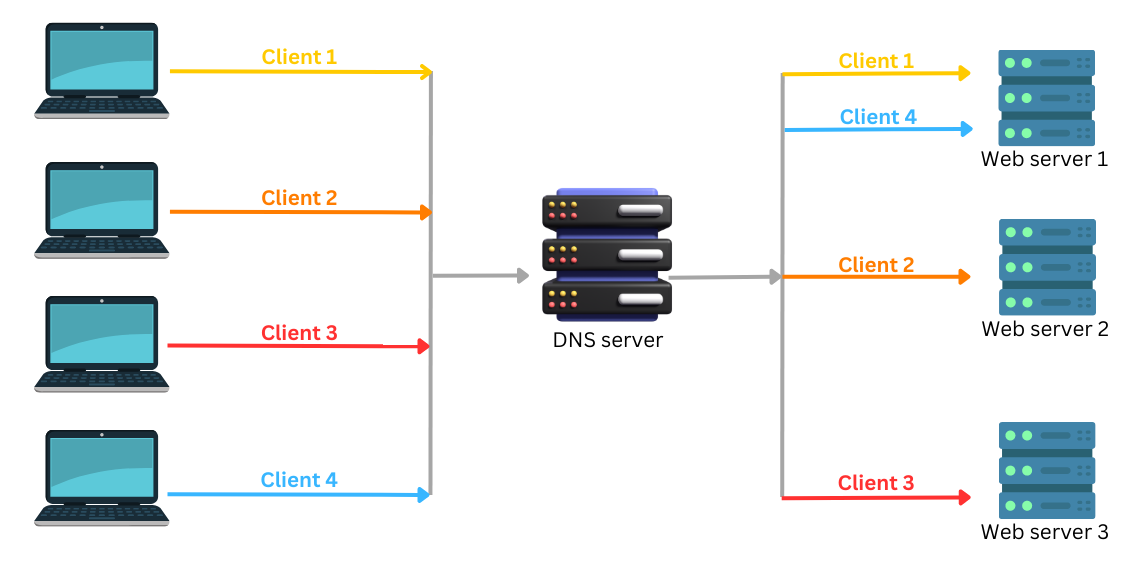
\includegraphics[width=\linewidth]{../images/roundrobindns}
  \caption{DNS Round Robin-Architektur~\cite{cloudns-roundrobin}}
    \label{fig:rrdns}
  \Description{Diagramm mit vier Clients, welche durch einen DNS-Server jeweils eine der vier Serveradressen primär nutzen}
\end{figure}

Das Domain Name System, kurz DNS, wird genutzt um eine Assoziation zwischen einer Domain und einer IP-Adresse zu hinterlegen.
Beispielsweise könnte ein Record hinterlegt werden, dass die Domain \verb|server.de| auf die Serveradresse des ersten Lastverteilers zeigt.
Wenn ein Client nun anstelle einer IP-Adresse die zugehörige Domain benutzt, wird zuerst der lokale DNS (Cache) befragt, ob der Name zu einer IP aufgelöst werden kann.
Ansonsten wird der externe autoritative Namensserver nach der IP befragt, und diese dann lokal zwischengespeichert und genutzt~\cite{Kopparapu.2002}.

Falls die IP des Lastverteilers nicht erreichbar ist, würde die Anfrage also fehlschlagen.
Es ist jedoch möglich, für eine Domain mehrere IP-Adressen zu hinterlegen.
Diese würden dann zu verschiedenen Servercomputern, ggf. mit jeweils eigenen internen Lastverteilern führen.

Wenn ein Client nun zur Namensauflösung den autoritativen DNS befragt, gibt dieser immer alle Records zurück.
Die Reihenfolge der IP-Adressen wird jedoch im Round Robin Verfahren zyklisch rotiert:
Wenn die erste Anfrage die drei Adressen \colorbox{lightgray}{A-B-C} erhält, würde die zweite Anfrage die Antwort \colorbox{lightgray}{B-C-A} erhalten.

So ist bereits für eine rudimentäre Lastverteilung gesorgt, da bei jeder Auflösung eine andere Adressreihenfolge herausgegeben und genutzt wird.
Auch die Verfügbarkeit ist erhöht, da ein Client bei Nichterreichbarkeit einer Adresse zur nächsten zurückgreifen kann.

\subsubsection{Vorteile}
DNS Round Robin hat zwei große Vorteile:
\begin{itemize}
	\item Es ist simpel zu implementieren, da keine spezielle Software auf dem Server- oder Clientsystem notwendig ist. Die Lastverteilung und Redundanz wird hier allein durch den Namensserver ermöglicht.
	\item Es schützt vor kompletter Nichterreichbarkeit. Ein Lastverteiler auf dem Server hilft nicht mehr wenn er selbst ausgefallen ist, oder wenn durch andere Probleme wie Geoblocks oder Firewalls gewisse IP-Ranges für den Client nicht erreichbar sind.
\end{itemize}

\subsubsection{Nachteile}
Auf den ersten Blick scheint dieses Verfahren ähnlich effektiv zu sein wie die statische Round Robin Lastverteilung aus Abschnitt \ref{sec:loadbalancing-strats}:
Anfragen werden ohne Einsicht in die Ressourcenverfügbarkeit möglichst fair auf Kapazitäten aufgeteilt.
Dies funktioniert in der Praxis jedoch nur eingeschränkt, da DNS-Einträge zwischengespeichert werden.
Die Lastverteilung erfolgt also nur in seltenen Abständen.
Besonders wenn regulär nur eine kleine Anzahl von Clients mit jeweils hohen Rechenanforderungen auf das System zugreifen,
kann schnell durch Zufall eine ungleiche Auslastung entstehen (eine große Nutzerzahl würde erhebliche Schwankungen eindämmen).

Dieses Problem kommt erneut ins Spiel, wenn einer Überlastung entgegengesteuert werden soll.
Nur neue Nutzer würden einen neu hinzugefügten DNS-Eintrag unmittelbar erhalten, wodurch eine erhebliche Verzögerung bis zur gleichverteilten Benutzung aller DNS-Einträge erfolgt.

Zuletzt ist auch das Verhalten im Fehlerfall nachteilhaft.
Zwei bestehende Probleme haben den Ursprung darin, dass der Client die Verantwortung für das Failover-Verhalten übernimmt:
\begin{itemize}
	\item Der Rückfall auf die weiteren IP-Adressen kann nur erfolgen, wenn der Client einen Fehler bei dem Abruf der Primäradresse erkennt. Dies funktioniert wenn der Server nicht erreichbar ist. Wenn aber stattdessen beispielsweise Fehlercodes anstatt von Inhalt zurückgegeben werden, ist die Kommunikation mit dem Host aus Sicht des Clients erfolgt; es erfolgt kein Failover.
	\item Der Client kann erst nach einer gewissen Wartezeit davon ausgehen, dass eine Adresse nicht erreichbar ist. So kann eine erhebliche Wartezeit entstehen, bis das Failover-Verhalten ausgelöst wird~\cite{so-dns-slow}.%\todo{n. d. schrott}
\end{itemize}

\subsubsection{Exkurs: Geolocation DNS}
Einige DNS-Anbieter unterstützen eine geolokalisierte DNS. Diese funktioniert aus Sicht des Clients und Servers sehr ähnlich zum beschriebenen DNS Round Robin. Anstelle die Adressen jedoch nur zyklisch herauszugeben, wird hier die IP-Adresse des anfragenden Clients herausgegeben. Mithilfe dieser kann ermittelt werden, aus welchem geografischen Raum die Anfrage kommt. Der DNS nutzt diese Information, um als Primäradresse die Adresse eines Servers zurückzugeben, welcher dem Client am nächsten ist \cite{mic-geodns}. 

So entsteht ein wichtiger Vorteil: Zum einen wird auch hier bereits die Last auf mehrere Server verteilt (darüberhinaus können GeoDNS und Round Robin auch kombiniert werden). Zum anderen wird aber auch der physische Abstand von Client und Server reduziert. Hohe Abstände führen zu deutlich höheren Latenzen, was insbesondere für Echtzeitaufgaben wie Sprachtelefonie oder Livestreaming nachteilhaft ist. Aber auch beispielsweise das Laden einer Webseite wird erheblich verlangsamt, besonders wenn viel Anfragen aufeinander aufbauen (also ein langer \textit{Request Waterfall} vorhanden ist).

Internationale Nutzer mit der gleichen Domain an verschiedene Zonen weiterzuleiten, kann die Leistung also erheblich erhöhen \cite{mic-geodns}.






